\documentclass[]{article}
\usepackage{amsmath}
\usepackage{tikz}
\usepackage{listofitems}
\usepackage{etoolbox}

\tikzset{>=latex}
\colorlet{myred}{red!80!black}
\colorlet{myblue}{blue!80!black}
\colorlet{mygreen}{green!60!black}
\colorlet{myorange}{orange!80!black}
\colorlet{myyellow}{yellow!80!black}

\colorlet{mydarkred}{myred!40!black}
\colorlet{mydarkblue}{myblue!40!black}
\colorlet{mydarkgreen}{mygreen!40!black}
\colorlet{mydarkorange}{myorange!40!black}
\colorlet{mydarkyellow}{myyellow!40!black}

\tikzset{
  node/.style={very thick,circle,draw=myblue,minimum size=22,inner sep=0.5,outer sep=0.6},
  input/.style={node,mydarkgreen,draw=mygreen,fill=mygreen!25},
  conv/.style={node,mydarkorange,draw=myorange,fill=myorange!25},
  flat/.style={node,mydarkyellow,draw=myyellow,fill=myyellow!25},
  dense/.style={node,mydarkblue,draw=myblue,fill=myblue!20},
  output/.style={node,mydarkred,draw=myred,fill=myred!20},
  connect/.style={-,thick,mydarkblue,shorten >=1}
}

\def\nstyle{%
  int(\lay==1 ? 1 : % Input
  (\lay<5 ? 2 :      % Conv layers
  (\lay==5 ? 3 :     % Flatten
  (\lay<8 ? 4 : 5))))} % Dense + Output

\title{\textbf{Document IA (faut trouver mieux comme nom)}} % TODO
\author{Pottier Loïc, Gros Charlène, Mudoy Jacques, Horter Louise, Los Thomas}
\date{\today}

\begin{document}

\maketitle


\section{Introduction}
Ce document fournit une présentation détaillée des architectures de réseaux de neurones utilisées pour jouer au jeu de plateau `Les tacticiens de Brême`. Il couvre la représentation des données d'entrée, le codage des sorties, le fonctionnement de l'apprentissage par renforcement profond (\textit{Deep Q-Learning}) ainsi que les différentes couches du réseau.
Nous étudierons d'abord le focntionnement du DQL avant de détailler les différents modèles utilisés.

\section{Le DQL}
blabla
% TODO expliquer le dql
% TODO expliquer que le système de récompense est traité dans le document sur le récompenses.

\section{Modèle 1} % TODO: Si on leur donne des noms c'est sympa
Ce premier modèle prend en entrée une représentation du plateau de jeu et produit une distribution sur les mouvements possibles.
Le modèle n'ayant pas connaissance des mouvements interdits, on utilise un masque pour les éviter.

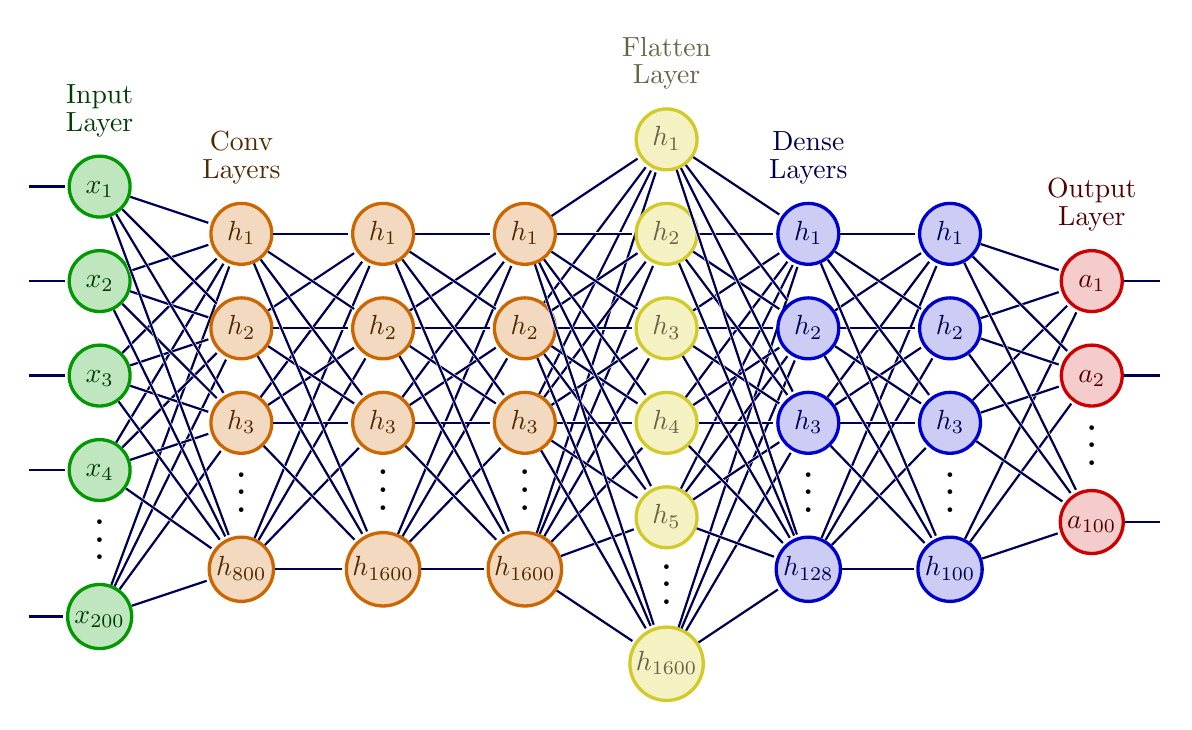
\begin{tikzpicture}[x=1.8cm,y=1.2cm]
    % Input: 5 nodes
    % Conv Layers (2-4): 32, 64, 64 nodes
    % Flatten Layer (5): 1600 nodes
    % Dense Layers (6-7): 128, 100 nodes
    % Output Layer (8): 100 nodes
    \readlist\Nnod{5,4,4,4,6,4,4,3} 
    
    \readlist\Nnode{200, 800, 1600, 1600,1600,128,100,100}  
    \readlist\Cstr{x,h,h,h,a,z,z,y} 
    
    \def\yshift{0.55}
    
    \foreachitem \N \in \Nnod{
        \def\lay{\Ncnt}
        \pgfmathsetmacro\prev{int(\Ncnt-1)}
        \foreach \i [evaluate={
            \c = int(\i==\N);
            \y = \N/2 - \i - \c * \yshift;
            \x = \lay;
            \n = \nstyle;
            \index = (\i<\N ? int(\i) : "\Nnode[\lay]");
        }] in {1,...,\N}{
            \pgfmathsetmacro\nstyle{int(\n==1 ? "input" : (\n==2 ? "conv" : (\n==3 ? "flat" : (\n==4 ? "dense" : "output"))))}
            \node[\nstyle] (N\lay-\i) at (\x,\y) {$\strut\Cstr[\n]_{\index}$};
            \ifnumcomp{\lay}{>}{1}{
                \foreach \j in {1,...,\Nnod[\prev]}{
                    \draw[white,line width=1.2,shorten >=1] (N\prev-\j) -- (N\lay-\i);
                    \draw[connect] (N\prev-\j) -- (N\lay-\i);
                }
                \ifnum \lay=\Nnodlen
                    \draw[connect] (N\lay-\i) --++ (0.5,0);
                \fi
            }{
                \draw[connect] (0.5,\y) -- (N\lay-\i);
            }
        }
        \path (N\lay-\N) --++ (0,1+\yshift) node[midway,scale=1.6] {$\vdots$};
    }
    \node[above=3,align=center,mydarkgreen] at (N1-1.90) {Input\\[-0.2em]Layer};
    \node[above=3,align=center,mydarkorange] at (N2-1.90) {Conv\\[-0.2em]Layers};
    \node[above=3,align=center,mydarkyellow] at (N5-1.90) {Flatten\\[-0.2em]Layer};
    \node[above=3,align=center,mydarkblue] at (N6-1.90) {Dense\\[-0.2em]Layers};
    \node[above=3,align=center,mydarkred] at (N8-1.90) {Output\\[-0.2em]Layer};
\end{tikzpicture}

\subsection{Représentation des Entrées}
Le plateau est représenté comme une grille \(5 \times 5\), où chaque case est encodée par un vecteur à 8 canaux décrivant la présence des différents pions.

\begin{itemize}
    \item Les 4 premiers canaux : Présence des pions bleues (\textit{âne\_bleu}, \textit{chien\_bleu}, \textit{chat\_bleu}, \textit{coq\_bleu}).
    \item Les 4 canaux suivants : Présence des pions rouges (\textit{âne\_rouge}, \textit{chien\_rouge}, \textit{chat\_rouge}, \textit{coq\_rouge}).
\end{itemize}

\paragraph{Exemple}

\begin{verbatim}
[0, 0, 1, 0, 1, 0, 0, 0] # chat bleu, âne rouge
[0, 0, 0, 0, 0, 0, 0, 0] # case vide
\end{verbatim}

\subsubsection{Dimensions des Entrées}
\begin{itemize}
    \item Pour un plateau unique : \((8, 5, 5)\) (canaux, lignes, colonnes).
    \item Pour un lot de plateaux (\textit{batch}) : \((\text{taille\_batch}, 8, 5, 5)\).
\end{itemize}

\subsection{Représentation des Sorties}
La sortie du réseau encode tous les déplacements possibles sous forme de liste aplatie de paires \((\text{pion}, \text{destination})\).

\subsubsection{Taille de la Sortie}
La sortie compte \(4 \times 25 = 100\) mouvements possibles :
\begin{itemize}
    \item 4 pions possibles (par joueur).
    \item 25 cases possibles (une grille \(5 \times 5\)).
\end{itemize}

\subsubsection{FAUT TROUVER UNE NOM} % TODO
Chaque index \(i\) dans la sortie correspond à :
\[
\text{index\_pion} = \frac{i}{25}, \quad
\text{ligne\_destination} = \frac{i \bmod 25}{5}, \quad
\text{colonne\_destination} = i \bmod 5.
\]

\subsubsection{Masquage}
Un masque binaire est appliqué aux 100 scores de sortie pour invalider les mouvements impossibles. Les mouvements invalides reçoivent un score de \(-\infty\) avant l'étape \textit{softmax} :
\begin{verbatim}
Masque = [0, 1, 0, ..., 1]  # 1 pour les mouvements valides, 0 sinon
\end{verbatim}

\subsection{Architecture du Réseau de Neurones}
L'architecture prend la représentation du plateau en entrée et produit une distribution sur les 100 mouvements possibles. Le réseau utilise des couches convolutionnelles pour extraire les caractéristiques spatiales, suivies de couches entièrement connectées pour produire les scores finaux.

\subsubsection{Entrée}
\(\text{Dimensions d'Entrée}: (\text{taille\_batch}, 8, 5, 5)\)

\subsubsection{Couches Convolutionnelles}
\begin{itemize}
    \item \(\text{Conv2D}(8 \rightarrow 32)\) \(\rightarrow\) ReLU
    \item \(\text{Conv2D}(32 \rightarrow 64)\) \(\rightarrow\) ReLU
    \item \(\text{Conv2D}(64 \rightarrow 64)\) \(\rightarrow\) ReLU
\end{itemize}

\subsubsection{Couches Entièrement Connectées}
\begin{itemize}
    \item \(\text{Flatten}\)
    \item \(\text{Linear}(5 \times 5 \times 64 \rightarrow 128) \rightarrow \text{ReLU}\)
    \item \(\text{Linear}(128 \rightarrow 100)\)
\end{itemize}

\subsubsection{Sortie}
\[
(\text{taille\_batch}, 100)
\]
Ce vecteur est ensuite combiné avec le \textit{masque} pour garantir que seuls les mouvements valides sont pris en compte.

\subsection{Limitations du Modèle}
\begin{itemize}
    \item \textbf{Dimensions fixes} : Les dimensions des entrées et des sorties doivent toujours rester constantes (\(8 \times 5 \times 5\) pour les entrées et \(100\) pour les sorties). Toute modification dans la taille du plateau ou le nombre de pions nécessiterait une révision complète du modèle.
\end{itemize}

\end{document}
